\title{VIMS Saturn Image-Mode Occultations Code Document}
\author{
        ASDF
}
\date{}

\documentclass[12pt]{article}

\usepackage{graphicx}
\graphicspath{{.}}

\begin{document}
\maketitle

\begin{abstract}
Cassini VIMS observed over 100 occultations by Saturn of background stars, a
handful of which were observed through a series of small-frame images instead
of a single spatial pixel pointed at the star's initial location on the sky.
These imaging-mode occultations provide a chance to directly observe the stars'
refraction through the outer layers of Saturn's atmosphere and constrain the
relative importance of differential refraction to other sources of attenuation
in the photometry of an occultation. Two critical steps that such an analysis
will rely upon are the correction of systematic and background signals in the
data, and carefully tracking the position of the star in the VIMS field.

There are three major sources of systematic background sources that we consider
in the current version of the code: an additive temporally-dependent background
level, an additive spatially-dependent background level, and a multiplicative
spatially-dependent sensitivity variability. These effects must be modeled and
removed before further work can begin. A multiplicative temporally-dependent
"ramp" effect is not observed, and not modeled.

A future background-correction method that we intend to implement into the code
calculates the position of the limb of Saturn as it progresses across the field
of view, and calculates the spatial background in that reference frame before
correcting it out.

Tracking the center of a star in a VIMS image is a difficult task because the
PSF of the star is less than one pixel. Still, the star is rarely centered in a
pixel, and so centering can be achieved by looking at how much light spills
into the pixels on either side of the brightest one along each axis.
Fortunately, the Pixel Response Function (PRF) is well-defined for the single
VIMS spatial pixel as a function of the angle between the center of the pixel
and the star. The experiment that characterized the PRF slewed the spacecraft
so that the star raster-scanned across the pixel. Refining the location of the
star relative to the pixel will also help us constrain the photometry because
we can calculate how the pixel's expected response will change as the star's
location moves across it.

\end{abstract}

\section{The Data}

\begin{figure}[h!]
  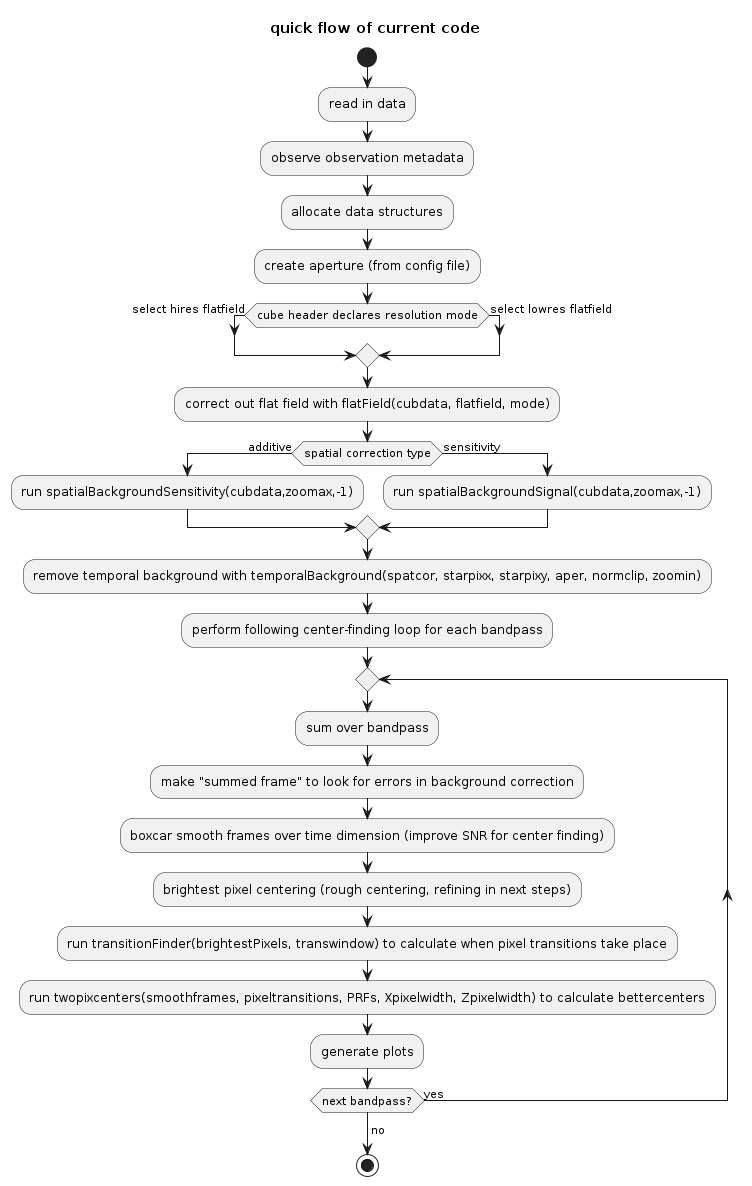
\includegraphics[width=0.7\linewidth]{codeflow.png}
  \caption{code flowchart for current version}
  \label{fig:flowchart}
\end{figure}

This section will describe what the raw data looks like in .cub format, and the
datastructures in the code that hold the data and analysis results. This will
be a quick reference area for which axis of which array corresponds to which
variable, or for the arguments of the various functions, etc. See
\ref{fig:flowchart} for a flowchart of the current data reduction procedure.

\subsection{cubdata}

{\bf cubdata} is the variable that holds the raw data from the cube files. It
is a four dimensional array.\\

{\it Axis 0} is the frame number, a proxy for time during the observation (a more
precise measurement of time can be found in the cubheader dictionary).\\

{\it Axis 1} is the spectral dimension, 256 channels.

{\it Axis 2 and 3} are the Z and X dimensions of the frame, respectively.

\section{The Code}

This section will contain an outline of the code and all relevant functions,
with relevant algebraic representations of each function and logic maps / flow
charts drawn out.

\subsection{Configuration File}

A basic overview of the configuration file's inputs is found in table
\ref{tab:configs}.\\

\begin{table}
\centering
\begin{tabular}[h!]{l|l|l}

variable   &    datatype    &   description\\
\hline
\hline
cubdir     &    string      &   location of .cub files\\
cubfiles   &    list of strings&list of the names of the .cub files\\
flatdir    &    string      &   location of flat files\\
PRFfile    &    string      &   location of PRF file\\
\hline
visible    &    boolean     &   are there visible data?\\
continua   &    tuple       &   what channels to look at\\
\hline
starpixx   &    tuple       &   x pixel range of the star for aperture\\
starpixy   &    tuple       &   y pixel range of the star for aperture\\
\hline
slope      &    float       &   urad/cube slope of line plotted\\
offset     &    float	    &   mrad offset of line\\
\hline
backgroundcheck&boolean     &   summing the background of the entire frame to \\
& & check for gradients, etc?\\
skipcol1   &    boolean     &   skip the first column when doing photometry?\\
\hline
spaback    &    string      &   "Sensitivity" or "Additive" - different ways of\\
& &  applying the spatial background correction\\
\hline
normclip   &    int         &   number of frames to clip for normalization of\\
& & spectrum (if first few are bad)\\
binning    &    int         &   number of cubes to bin temporally for binned\\
& & spectra\\
smooth     &    int         &   number of frames to smooth together for \\
& & rolling average for center-finding algorithm\\
transwindow&    int         &   windowsize for pixel transitions finder\\
\hline
zoomin     &    int         &   lower bound for zoomed plots\\
zoomax     &    int         &   upper bound for zoomed plots\\
\hline
movies     &    boolean     &   generate movies? (takes a LONG time)\\
gamma      &    float, [0,1]&   gamma stretch of output frames\\
\hline
\end{tabular}
\caption{Table of Configuration File Parameters}
\label{tab:configs}
\end{table}


\subsection{Occultation Functions}

{\it \noindent def readVIMSimaging(cubdir, cubfiles, ncubs, nspec, height, width, visible):}\\

  Reads in vims cub files\\

{\it \noindent def flatField(cubdata, flatfield, mode):}\\

  Reads in the official VIMS flatfield file, and uses it to correct the cubdata
  (simple division)\\

{\it \noindent def spatialBackgroundSignal(cubdata, start, end):}\\

  subtracts the average value of each pixel as a spatial background subtraction
  under the assumption that this average brightness is an extra physical signal
  \\

{\it \noindent def spatialBackgroundSensitivity(cubdata, start, end):}\\

  see above, but dividing out each pixel's average deviation from the the median
  frame, normalized such that the median is 1.\\

{\it \noindent def temporalBackground(data, starpixx, starpixy, aper, normclip, zoomin):}\\

  takes the median of each frame at each wavelength outside of the aperture
  and subtracts that value from the frame.\\
  This function also returns a version normalized in each channel to the average
  value in that channel between normclip and zoomin\\

{\it \noindent def transitionfinder(list, window, xpositive = True, Zpositive = True):}\\

  list is the list of brightest pixels. Window is the window that we look at
  finds the mode of brightest pixels within a window surrounding the current
  pixel. Returns a list of indices at which this mode transitions\\

{\it \noindent def twopixcenters(data, transitions, PRFs, xwidth, Zwidth):}\\

  this function is dominated by a for loop over the frames. It also keeps
  track of a "step" counter. step starts at 0 and increments every time that
  a "transition" frame is reached per the transitions array inputted. For each
  step, the current mode-brightest-pixel is compared to the brightest pixel on
  the other side of the nearest transition by the math:\\
    comparisonpixel/brightestpixel\\
  This "metric" is then compared to a similar metric from the PRF pixel scans:\\
    pixelscanshiftedbyonepixelwidth / pixelscan\\
  the pixel scan is shifted (np.roll) by one pixel width and divided by itself.
  the direction of the shift is determined by whether the compare pixel is to
  the left or right of the mode-brightest.\\
  the sub-pixel position on the PRF scan with the metric closest to the
  "empirical" metric calculated from the dataframe is called the "correction"
  this correction is added to the current mode-brightest and returned as the
  new center of star in that frame.\\


\subsection{Code File}

\subsubsection{Initialization}

imports code of config file\\

Opens first cub file for information about shape, observing mode, etc
Allocates space for reading in the rest\\

Tries opening the data from a save file, if it fails, it reads in the data from
the .cub files\\

Reads header for mode information, sets pixel widths and flatfield location.\\

Reads in PRF scans\\

creates simple box aperture bounded by starpixx and starpixy\\
{\bf NOTE:} I have also added a "panhandle" to this aperture box in some previous
iterations, this line is currently commented out\\

allocates arrays for things\\

\subsubsection{Background Correction}

First step is subtracting the official VIMS flatfield (see oF.flatField)

Second we either subtract or divide out the spatial background gradient
(see oF.spatialBackgroundSensitivity and/or oF.spatialBackgroundSignal)

Third, we subtract out the temporal background

TODO: try to combine steps 2 and 3 here

\subsubsection{Looping Over Bandpasses}

The following is a series of actions that we perform on each of the
predetermined bandpasses:

\begin{enumerate}
\item Make a new set of "frames" summed over the given bandpass
\item if backgroundcheck == True:
   \begin{itemize}
   \item sum all of these frames to get the average value of each pixel to test
      spatial background correction
   \end{itemize}
\item Smooth frames in time with a window size of "smooth"
\item Mark the brighest pixel in the smoothed frame
\item use transitionfinder to find the transitions in the brightestPixel array
\item use bettercenters to calculate finer-grained centering
\end{enumerate}

\subsubsection{COMINGSOON: Better Photometry Using Center Locations}

Going to test three different methods of photometry:
\begin{enumerate}
\item only taking photometry of the brightest pixel, and only when the star is
   near the center of the pixel
\item only taking photometry of the brightest pixel, scaled by the PRF scan based
   on the center location within the pixel
\item using a moving, fuzzy aperture
\end{enumerate}


\section{The Plots}

This section will describe the plots generated by the code and what information
they each plot, with examples of each.

\end{document}
This is never printed
